% !TEX root = ../../main.tex

\section{Experimental Setup}
\label{app:experimental}

\subsection{Datasets}
\label{app:experimental-datasets}

\headernodot{Flickr30k} consists of \numprint{31000} images annotated with 5 matching captions~\citep{young2014image}. 

\headernodot{MS-COCO} consists of \numprint{123287} images, each image annotated with 5 matching captions~\citep{lin2014microsoft}.  
The original dataset was introduced for large-scale object recognition.

For both datasets, we use the training, validation, and test splits from~\citep{karpathy2015deep}.

\subsection{Models}
\label{app:experimental-models}

We use CLIP and VSE++. Both consist of an image and a text encoder that do not share parameters.

\headernodot{CLIP} is a large-scale image-text foundation model~\citep{radford2021learning}.
The model is pre-trained on a collection of \numprint{400} million image-text pairs collected from the Web. 
The encoders are pre-trained using a contrastive loss (InfoNCE) on image-text pairs.
The text encoder of consists of a 12-layer transformer model, described in~\citep{radford2019language}.
As for the image encoder, CLIP utilizes various model backbones, such as ResNet~\citep{he2016deep}  and Vision Transformer~\citep{dosovitskiy2021image}.
In this work, we use the ResNet-50  (‘RN50’) variant of the CLIP image encoder.\footnote{\url{https://github.com/openai/CLIP/}}
The CLIP encoders are trained to jointly understand images and text.
Therefore, the learned representations generalize to a wide range of different zero-shot (visual) evaluation tasks, such as classification, without task-specific fine-tuning, by using textual prompts. 

\headernodot{VSE++} is an image-caption encoder trained from scratch~\citep{faghri2018improving}.
The model features a triplet loss function with a margin parameter $\alpha=0.2$.
The text encoder is a one-layer gated recurrent unit (GRU)~\citep{cho2014_learning}.
The available image encoder configurations are ResNet-152~\citep{he2016deep} and VGG19~\citep{simonyan2015_very_deep}.
In this work, we use ResNet-152.

\subsection{Training}
\label{app:experimental-training}

\header{CLIP} To fine-tune CLIP, we follow~\citep{yuksekgonul2023when}.
All models are fine-tuned for 5 epochs.
We employ a cosine-annealing learning rate schedule, with a base learning rate of $2e-5$, and 100 steps of warm-up.
As an optimizer, we use AdamW~\citep{loshchilov2019decoupled} with a gradient clipping value of $2$.
For the InfoNCE loss, we use the logit-scale (i.e., temperature $\tau$) from the pre-trained CLIP model and fine-tune the logit-scale end-to-end along with the rest of the model parameters.

\header{VSE++} The model is trained for 30 epochs using a linear learning rate schedule with a base learning rate of $2e-4$. We use the Adam optimizer~\citep{kingma2014_adam} with a gradient clipping value of $2$. Instead of the triplet loss, we use the InfoNCE loss similar to~\cite{radford2021learning},

For both models, instead of selecting the best-performing model based on the validation set scores, we use the final checkpoint at the end of training. 


\subsection{Shortcut Sampling}
\label{app:experimental-shortcutsampling}

Our goal is to add the shortcuts in a manner that preserves the original information of the images and captions. 
For the captions, we append the shortcut at the end of the captions.
In order to prevent a tokenizer from tokenizing the shortcut into a single token, we insert spaces between each number of the shortcut.
For the images, we place the numbers of the shortcuts at the top of the images, evenly spaced across the entire width of the images (to make sure the shortcut is evenly spaced across the feature map of the image).
We always use 6 digits to represent a shortcut.  
If a shortcut number contains fewer than 6 digits, we fill the remaining positions with zeros for padding.
For the MNIST images, we always sample a random image from the set of images representing the number that belongs to (also during evaluation), to prevent overfitting on specific MNIST images. 
In Figure~\ref{fig:shortcut_examples}, we provide four examples of image-caption pairs with randomly added shortcuts. 
The examples in Figure~\ref{fig:shortcut_examples} show 
\begin{enumerate*}[label=(\roman*)]
	\item how synthetic shortcuts are added to the image and the caption, and 
	\item that the shortcuts preserve the original (task-relevant) information of the images and captions.
\end{enumerate*}

\begin{figure}[t!]
	\centering
	\begin{subfigure}[b]{0.475\textwidth}
		\centering
		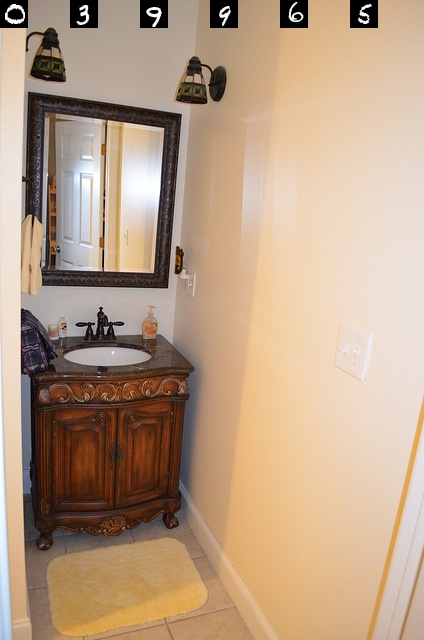
\includegraphics[width=\textwidth, height=\textwidth]{figures/shortcut_examples/shortcut_img1.jpg}
		\caption{\textbf{Caption}: ``A bathroom sink with wood finish cabinets.  0 3 9 9 6 5.''}%
		\label{fig:shortcut1}
	\end{subfigure}
	\hfill
	\begin{subfigure}[b]{0.475\textwidth}  
		\centering 
		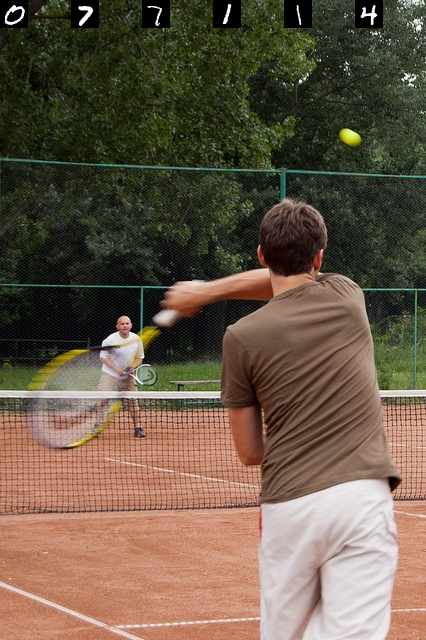
\includegraphics[width=\textwidth, height=\textwidth]{figures/shortcut_examples/shortcut_img2.jpg}
		\caption{\textbf{Caption}: ``A guy in a brown shirt has just hit a tennis ball.  0 7 7 1 1 4.''}%  
		\label{fig:shortcut2}
	\end{subfigure}
	\vskip\baselineskip
	\begin{subfigure}[b]{0.475\textwidth}   
		\centering 
		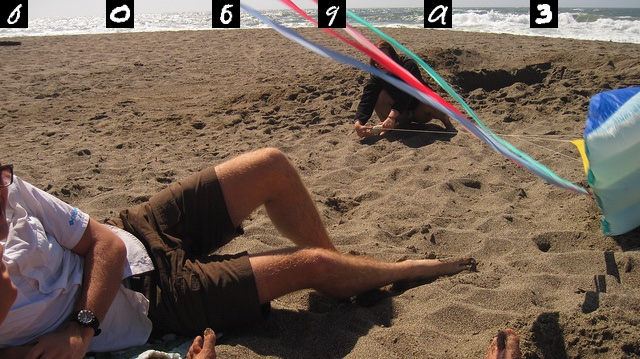
\includegraphics[width=\textwidth, height=\textwidth]{figures/shortcut_examples/shortcut_img3.jpg}
		\caption{\textbf{Caption}: ``A man in shorts is lying on the beach. 0 0 6 9 9 3.''}% 
		\label{fig:shortcut3}
	\end{subfigure}
	\hfill
	\begin{subfigure}[b]{0.475\textwidth}   
		\centering 
		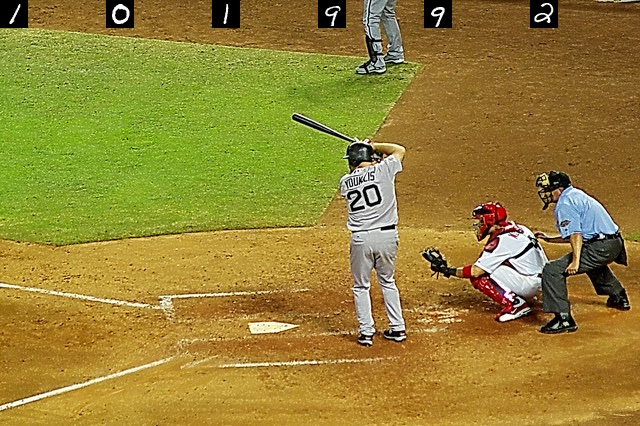
\includegraphics[width=\textwidth, height=\textwidth]{figures/shortcut_examples/shortcut_img4.jpg}
		\caption{\textbf{Caption}: ``A player up to bat in a baseball game. 1 0 1 9 9 2.''}%
		\label{fig:shortcut4}
	\end{subfigure}
	\caption{Four random samples from the \acs{MS-COCO} dataset including shortcuts added on both the image and caption.
	}
	\label{fig:shortcut_examples}
\end{figure}
